The effect of the number of training samples used for the creation of feature histograms is displayed in table \ref{tab:size_hist}. The results show that the Mean Average Precision increases when more training samples per class are used. This is because the visual vocabulary is formed with feature histograms which are more generalizing and thus the image features are more descriptive for each classifier. Figure \ref{fig:size_hist} shows clearly that the performance of the automated image classification stabilizes as the training samples size reaches approximately 70 images per class. This training sample size is sufficient for the generalization of feature histograms and enlarging the training sample size will not increase performance significantly. 

\begin{figure}[H]
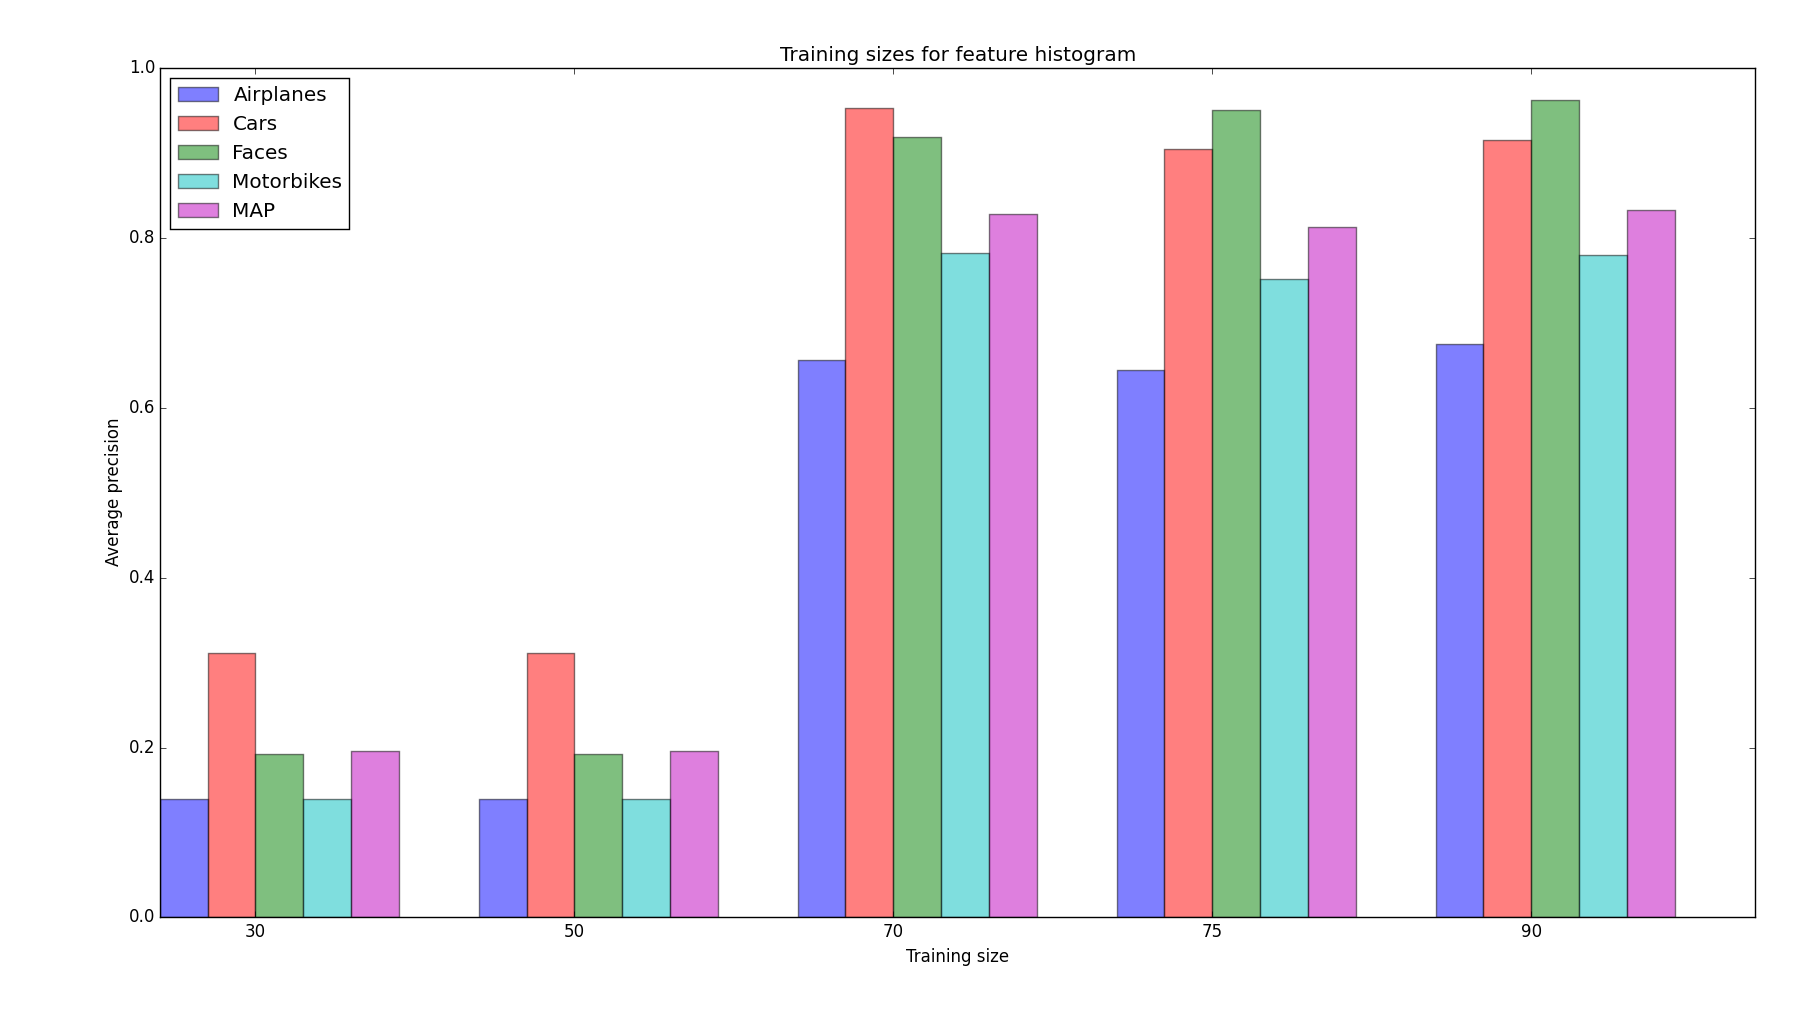
\includegraphics[width=\textwidth]{../plots/training_size_feature_histograms}
\caption{Effect of training size for histograms on AP}
\label{fig:size_hist}
\end{figure}

\begin{table}[H]
\begin{tabular}{|c|ccccc|}
\hline
\textbf{Training samples} & \textbf{AP Airplanes} & \textbf{AP Cars} & \textbf{AP Faces} & \textbf{AP Motorbikes} & \textbf{MAP}\\
\hline
30 & 0.1394 & 0.3118& 0.1924& 0.1394 & 0.1958\\
50 & 0.1394 & 0.3118& 0.1924& 0.1394 & 0.1958\\
60 & 0. & 0. & 0. & 0. & 0.\\
70 & 0.6563 & 0.9534 & 0.9191 & 0.7830 & 0.8280\\
75 & 0.6447 & 0.9053 & 0.9510 & 0.7516 & 0.8132\\
90 & 0.6749 & 0.9157 & 0.9631 & 0.7798 & 0.8334\\
\hline
\end{tabular}
\caption{Effect number of training samples (per class) for feature histogram, Sift type: dense, Color space: opponent}
\label{tab:size_hist}
\end{table}
